% MIT License

% Copyright (c) 2022 Chiyuru

% Permission is hereby granted, free of charge, to any person obtaining a copy of this software and associated documentation files (the "Software"), 
% to deal in the Software without restriction, including without limitation the rights
% to use, copy, modify, merge, publish, distribute, sublicense, and/or sell
% copies of the Software, and to permit persons to whom the Software is
% furnished to do so, subject to the following conditions:

% The above copyright notice and this permission notice shall be included in all copies or substantial portions of the Software.

% THE SOFTWARE IS PROVIDED "AS IS", WITHOUT WARRANTY OF ANY KIND, EXPRESS OR IMPLIED, INCLUDING BUT NOT LIMITED TO THE WARRANTIES OF MERCHANTABILITY,
% FITNESS FOR A PARTICULAR PURPOSE AND NONINFRINGEMENT. IN NO EVENT SHALL THE AUTHORS OR COPYRIGHT HOLDERS BE LIABLE FOR ANY CLAIM, DAMAGES OR OTHER
% LIABILITY, WHETHER IN AN ACTION OF CONTRACT, TORT OR OTHERWISE, ARISING FROM,
% OUT OF OR IN CONNECTION WITH THE SOFTWARE OR THE USE OR OTHER DEALINGS IN THE SOFTWARE.

% 宏定义一些数学符号

\def\f#1#2{\frac{#1}{#2}}
\def\d#1{\dot{#1}}
\def\dd#1{\ddot{#1}}
\def\fd#1#2{\frac{d #1}{d #2}}
\def\fp#1#2{\frac{\partial #1}{\partial #2}}
\def\b#1{\boldsymbol{#1}}


\documentclass[UTF8]{ctexart}

\usepackage{tikz}
\usetikzlibrary{3d,quotes,angles}
\usepackage{amsmath}
\usepackage{cases}
\usepackage{cite}
\usepackage{graphicx}
\usepackage[margin=1in]{geometry}
\geometry{a4paper}
\usepackage{fancyhdr}
\pagestyle{fancy}
\fancyhf{}

\title{SRT创新计划专项结题报告\\倒立摆控制}
\author{刘锦坤}
\date{\today}
\pagenumbering{arabic}

\begin{document}

%\fancyhead[L]{驰雨Chiyuru}
\fancyhead[C]{倒立摆控制}
\fancyfoot[C]{\thepage}

\maketitle
\tableofcontents
\newpage

\section{摘要}

在本次SRT项目中主要完成了利用PD控制器对倒立摆进行控制。但是在传统的PD控制中,PD控制的各个参数往往难以确定,需要大量的时间和精力调节。而本次SRT中完成了利用模块叠加法从理论上计算PD控制器的参数。
为此,首先通过第二类Lagrange方程建立了倒立摆的动力学模型,然后分析了倒立摆在$\theta = 0$下的本征模块。
随后设计PD控制器,并且利用模块叠加方法确定了PD控制器参数的稳定域,解释了PD控制中各个参数的来源。

\section{PD控制参数的理论计算}

在本次SRT项目中,选用PD方法来完成对倒立摆的控制,可以建立动力学模型,对PD控制器的参数进行理论计算。

\subsection{动力学方程}

系统动力学模型示意图如图所示:

\begin{figure}[htbp]
    \centering
    \begin{tikzpicture}[x={(-1cm,-1cm)},y={(1.5cm,0cm)},z={(0cm,1.5cm)}]
        % 定义坐标轴
        \draw[->] (0,0,0) -- (4,0,0) node[below] {$X$};
        \draw[->] (0,0,0) -- (0,4,0) node[right] {$Y$};
        \draw[->] (0,0,0) -- (0,0,4) node[above] {$Z,z$};
        % 画水平杆子
        \draw[line width=3pt] (0,0,0) -- (3,3,0) node[below] {$m_1,l_1$};
        % 画竖直虚线
        \draw[dashed] (3,3,0) -- (3,3,4);
        % 画竖直杆子
        \draw[line width=3pt] (3,3,0) -- (2,5,4) node[above] {$m_2,l_2$};
        % 两杆铰接处
        \draw[fill=black] (3,3,0) circle (0.05);
        % 标记phi角和tau
        \draw[thick,->] (0.5,0,0) arc (0:40:0.5 and 0.5);
        \node[font=\LARGE] at (0.9,0.4,0) {$\alpha,\tau$};
        % 标记theta角
        \draw[thick,->] (3,3,1) arc (0:35:-1.0 and 1.0);
        \node[font=\LARGE] at (3,3.3,1.2) {$^\theta$};
        % 随杆坐标轴
        \draw[->] (0,0,0) -- (4.3,4.3,0) node[below] {$x$};
        \draw[->] (0,0,0) -- (-2.5,2.5,0) node[above] {$y$};
        \draw[->] (0,0,0) -- (0,0,4);
    \end{tikzpicture}
    \caption{倒立摆示意图}
\end{figure}

$XYZ$坐标系为固定坐标系,而$xyz$为随着水平杆转动的坐标系。记水平杆的质量$m_1$,长度$l_1$,树枝干的质量$m_2$,长度$l_2$,水平杆的转动角度为$\alpha$,竖直杆的转动角度$\theta$,假设两杆的质量都是均匀分布。电机的驱动力矩为$\tau$,重力加速度为$g$,下面从第二类Lagrange方程出发推倒倒立摆的动力学方程。

水平杆的动能为

\begin{equation}
    T_1 = \f 1 6 m_1 l_1^2 {\d{\alpha}}^2
\end{equation}

竖直杆的动能为为质心动能和相对之心动能之和,其质心速度为:

\begin{equation}
    \vec v = -\f 1 2 l_2 \d{\alpha} sin \theta \hat x
    +(\d{\alpha} l_1+\f 1 2 l_2 \d{\theta} cos \theta )\hat y
    - \f 1 2 l_2 \d{\theta} sin \theta \hat z 
\end{equation}

其中$\hat{x},\hat{y},\hat{z}$为$xyz$坐标系各个方向的单位矢量,故其质心动能为

\begin{equation}
    \begin{aligned}
    T_{2c} &= \f 1 2 m_2 \vec v^2\\ 
    &= \f 1 2 m_2 {l_1}^2 {\d \alpha}^2
    +\f 1 2 m_2 \d \alpha \d \theta l_1 l_2 cos \theta
    +\f 1 8 m_2 {l_2}^2 {\d \theta}^2
    +\f 1 8 m_2 {l_2}^2 {\d \alpha}^2 sin^2 \theta
    \end{aligned}
\end{equation}

而竖直杆的相对质心动能为转动贡献,即为

\begin{equation}
    T_{2r} = \f {1} {24} m_2 l_2^2 {\d \theta}^2+ \f {1} {24} m_2 l_2^2 {\d \alpha}^2 sin^2 \theta
\end{equation}

系统势能为

\begin{equation}
    V = \f 1 2 m_2 g l_2 cos \theta
\end{equation}

系统的Lagrange量为

\begin{equation}
    \begin{aligned}
        L &= T - V = T_1 + T_{2c} + T_{2r} - V\\
        &= \f 1 6 m_1 l_1^2 {\d{\alpha}}^2
        +\f 1 2 m_2 {l_1}^2 {\d \alpha}^2
        +\f 1 2 m_2 \d \alpha \d \theta l_1 l_2 cos \theta
        +\f 1 8 m_2 {l_2}^2 {\d \theta}^2\\
        &+\f 1 8 m_2 {l_2}^2 {\d \alpha}^2 sin^2 \theta
        +\f {1} {24} m_2 l_2^2 {\d \theta}^2
        + \f {1} {24} m_2 l_2^2 {\d \alpha}^2 sin^2 \theta
        -\f 1 2 m_2 g l_2 cos \theta
    \end{aligned}
\end{equation}

保留到二阶小量,可以得到:

\begin{equation}
    L = \f 1 6 m_1 l_1^2 {\d{\alpha}}^2
    + \f 1 2 m_2 {l_1}^2 {\d \alpha}^2
    + \f 1 2 m_2 \d \alpha \d \theta l_1 l_2
    + \f 1 8 m_2 {l_2}^2 {\d \theta}^2
    + \f {1} {24} m_2 l_2^2 {\d \theta}^2
    + \f 1 4 m_2 g l_2\theta^2
\end{equation}

带入第二类Lagrange方程,得到

\begin{equation}
    \begin{cases}
        \f 1 3 m_1 l_1^2 \dd{\alpha} + m_2 l_1^2 \dd{\alpha} + \f 1 2 m_2 l_1 l_2 \dd{\theta} = \tau\\
        \f 1 2 m_2 l_1 l_2 \dd{\alpha} + \f 1 3 m_2 l_2^2 \dd\theta - \f 1 2 m_2 g l_2 \theta = 0
    \end{cases}
\end{equation}

记$\b{q}=[\alpha , \theta]^T$,有

\begin{equation}
    \b{M} \b{\dd q} + \b{K} \b{q} = \b{\tau}
\end{equation}

其中

\begin{equation}
    \b M = \begin{bmatrix}
        \f 1 3 m_1 l_1^2 + m_2 l_1^2 & \f 1 2 m_2 l_1 l_2\\
        \f 1 2 m_2 l_1 l_2  & \f 1 3 m_2 l_2^2
    \end{bmatrix},
    \b K = \begin{bmatrix}
        0 & 0\\
        0 & -\f 1 2 m_2 g l_2
    \end{bmatrix},
    \b \tau = \begin{bmatrix}
        \tau\\
        0
    \end{bmatrix}
\end{equation}

这就是倒立摆的动力学方程。

\subsection{本征模块}

我们先分析系统的本征模块,设其一个本征模块为$\b q(t) = \b{\eta_i} e^{\lambda_i t}$,代入方程$\b{M} \b{\dd q} + \b{K} \b{q} = 0$得到:

\begin{equation}
        \det(\lambda_i^2\b M + \b K)\b{\eta_i} = 0
\end{equation}

解特征方程得到其特征值

\begin{equation}
    \lambda_1 = 0, \lambda_2 = \pm \sqrt{\frac{6 (m_1+3 m_2)g}{(4 m_1+3 m_2) l_2}}
\end{equation}

对应的特征向量为

\begin{equation}
    \b \eta = [\b \eta_1, \b \eta_2]
\end{equation}

其中

\begin{equation}
    \b \eta_1 = \begin{bmatrix}
        \frac{\sqrt{3}}{\sqrt{(m_1+3m_2)l_1^2}}\\
        0
    \end{bmatrix},
    \b \eta_2 = \sqrt{\f{12(m_1+3m_2)}{m_2(4m_1+3m_2)l_2^2}}\begin{bmatrix}
        -\f{3m_2l_2}{2(m_1+3m_2)l_1}\\
        1
    \end{bmatrix}
\end{equation}

由于存在一个$\lambda_2$的实部大于0,这表明倒立摆的本征模块不是稳定的,因此需要进行控制。

\subsection{PD控制器}

接下来,我们用模块叠加方法来设计PD控制器\footnote{参考了赵治华老师《动力学于控制》课程讲义},我们实际可调节输入为$\tau$,控制变量为$\theta,\alpha$,因此实际上这是一个欠驱动问题,先用模块分解法将方程(9)进行处理,设$\b{q(t)}=\b{\eta}\b{s(t)},\b{s(t)}=[s_1(t),s_2(t)]^T$带入方程(9),再左乘$\b{\eta}^{T}$,得到

\begin{equation}
    \begin{cases}
        \dd{s_1}  -\eta_{11}\tau = 0\\
        \dd{s_2} - \lambda_2^2 s_2- \eta_{21}\tau = 0
    \end{cases}
\end{equation}

且有

\begin{equation}
    \begin{cases}
        \alpha(t) = \eta_{11}s_1(t) + \eta_{21}s_2(t)\\
        \theta(t) = \eta_{21}s_2(t)
    \end{cases}
\end{equation}

设置控制器为
\begin{equation}
    \eta_{21}\tau = -k_1 s_1 - k_2 s_2 - c_1 \d{s_1} - c_2 \d{s_2} -\lambda_2^2\d{s_2}
\end{equation}

并记$\mu = \eta_{11}/\eta_{21}$,代入方程(15)得到

\begin{equation}
    \begin{cases}
        \dd{s_1}-\mu\dd{s_2}+\mu\lambda_2^2 s_s = 0\\
        \dd{s_2}+k_2 s_2+c_2 \d{s_2}+k_1 s_1+c_1 \d{s_1}=0
    \end{cases}
\end{equation}

写为矩阵形式

\begin{equation}
    \b{M_s} \b{\dd s}+\b{C_s}\b{\d{s}}+\b{K_s} \b{s} = 0
\end{equation}

其中

\begin{equation}
    \b{M_s} = \begin{bmatrix}
        1 & -\mu\\
        0 & 1
    \end{bmatrix},
    \b{C_s} = \begin{bmatrix}
        0 & 0\\
        c_1 & c_2
    \end{bmatrix},
    \b{K_s} = \begin{bmatrix}
        0 & \mu\lambda_2^2\\
        k_1 & k_2
    \end{bmatrix}
\end{equation}

我们期望这样的控制器能够使得系统稳定,因此我们需要对于新的模块$\b{s(t)}=\b{\xi}e^{\beta_i t}$所有的$\beta_i$的实部均小于0.因此我们需要满足

\begin{equation}
    \det(\beta^2\b{M_s}+\beta\b{C_s}+\b{K_s}) = 0
\end{equation}

的$\beta_i$的实部全部小于0,这样我们就可以得到合适的$k_1,k_2,c_1,c_2$。由于我们知道在临界阻尼时,系统的衰减速度最快,因此我们可以设定上述特征方程的解是两个负的重实根$\beta_1,\beta_2$,即

\begin{equation}
    (\beta - \beta_1)^2(\beta-\beta_2)^2=0
\end{equation}

对比方程(21),(22)可以得到

\begin{equation}
    \begin{cases}
        k_1 = -\f{\beta_1^2\beta_2^2}{\mu\lambda_2^2}\\
        c_1 = \f{2\beta_1\beta_2(\beta_1+\beta_2)}{\mu\lambda_2^2}\\
        k_2 = \beta_1^2+\beta_2^2+4\beta_1\beta_2+\f{\beta_1^2\beta_2^2}{\lambda_2^2}\\
        c_2 = -2(\beta_1+\beta_2)-2\f{2\beta_1\beta_2}{\lambda_2^2}
    \end{cases}
\end{equation}

利用方程

\begin{equation}
    \begin{aligned}
        \tau &= -\f{1}{\eta_{21}}([k_1,k_2+\lambda_2^2]\b{s} + [c_1,c_2]\d{\b{s}}\\
        &= -\f{1}{\eta_{21}}([k_1,k_2+\lambda_2^2]\b{\eta}^{-1}\b{q} + [c_1,c_2]\b{\eta}^{-1}\d{\b{q}})
    \end{aligned}
\end{equation}

就能得到PD控制器的参数$K_{p\alpha},K_{p\theta},K_{d\alpha},K_{d\theta}$

\begin{equation}
    \begin{cases}
        \b{K_p}=[K_{p\alpha},K_{p\theta}]
        =-\f{1}{\eta_{21}}[k_1,k_2+\lambda_2^2]\b{\eta}^{-1}\\
        \b{K_d}=[K_{d\alpha},K_{d\theta}]
        =-\f{1}{\eta_{21}}[c_1,c_2]\b{\eta}^{-1}
    \end{cases}
\end{equation}

其中$\b{\eta}^{-1}$可以算出为

\begin{equation}
    \b\eta^{-1} =
\begin{bmatrix}
 \frac{l_1^2 (m_1+3 m_2)}{\sqrt{3} \sqrt{l_1^2 (m_1+3 m_2)}} & \frac{\sqrt{3} l_1 l_2 m_2}{2 \sqrt{l_1^2 (m_1+3 m_2)}} \\
 0 & \frac{l_2^2 m_2 (4 m_1+3 m_2)}{2 \sqrt{3} (m_1+3 m_2) \sqrt{\frac{l_2^2 m_2 (4 m_1+3 m_2)}{m_1+3 m_2}}} \\
\end{bmatrix}
\end{equation}

至此,我们就完成了倒立摆的PD控制参数的理论计算,只要我们选定两个负实数根$\beta_1,\beta_2$,就能计算得到合适的PD控制参数使得倒立摆在$\theta = 0$稳定。

\newpage

\section{基于Simulink的控制及理论验证}

\subsection{Simulink程序说明}

如图所示的Simulink程序成功的完成了对倒立摆的控制:

\begin{figure}[htbp]
    \centering
    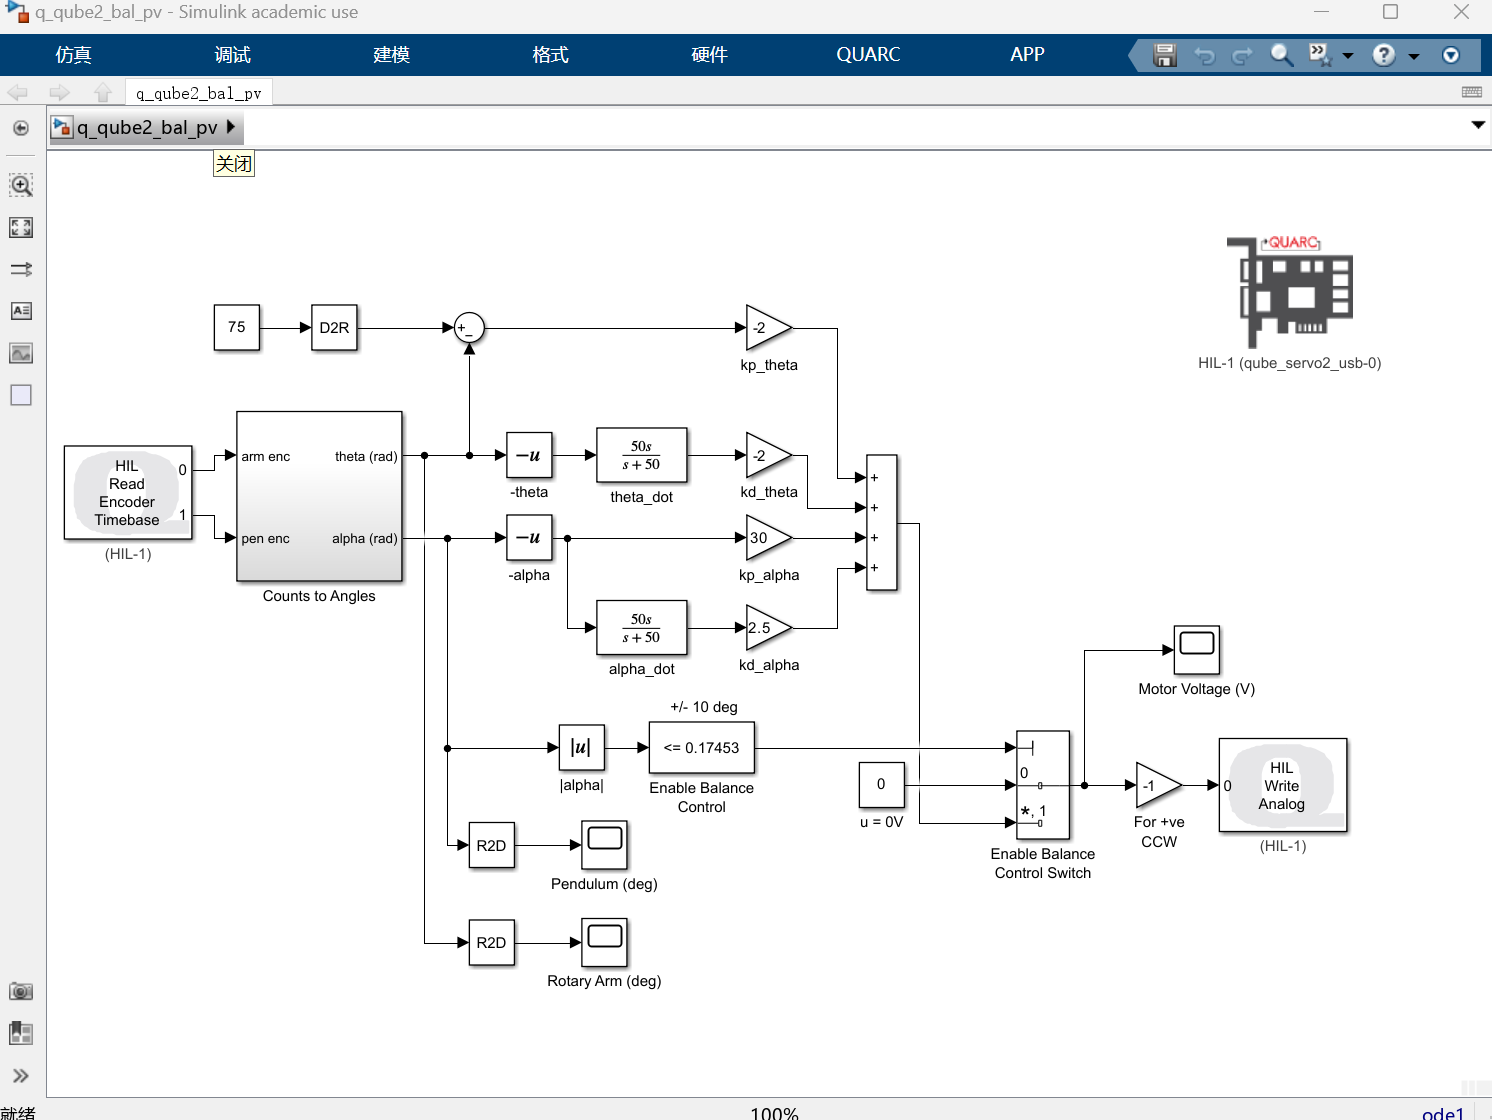
\includegraphics[width=0.8\textwidth]{Simulink.png}
    \caption{Simulink模型}
\end{figure}

程序在$|\theta|<10°$时启动PD控制,中从倒立摆的Encoder中读取得到$\alpha,\theta$,并由传递函数$\frac{50s}{s+50}$滤波后得到$\d{\alpha},\d{\theta}$,然后经过PD控制器得到$\tau$,作为倒立摆的输入,实现对倒立摆的倒立控制。

\subsection{PD参数的理论解释}

注意到在Simulink程序中,PD控制参数中的$K_{p\theta},K_{d\theta}$两项为负,而$K_{p\alpha},K_{d\alpha}$两项为正,
这个符号特性并不是偶然的,事实上这时方程(23)的结果,在方程(23)中可以看出,$k_1,c_1<0$而$k_2,c_2>0$,因此经过方程(25)的计算,$K_{p\theta},K_{d\theta}$两项为负,而$K_{p\alpha},K_{d\alpha}$两项为正。

\section{结论}

本次SRT项目中,成功的利用模块叠加法计算了PD控制器的参数。也在Simulink程序中成功的验证了计算得到的PD控制器的参数的正确性,实现了对倒立摆的控制。

值得注意的是,模块叠加法的思想是将一个复杂的系统分解为多个简单的模块,这其实是振动理论中简正模块的思想。这种方法也可以用于分析其他的控制问题,其基本思路如下:

\begin{enumerate}
    \item 建立系统的动力学模型,并且计算得到系统的动力学方程,在控制稳定点附近进行线性化
    \item 计算线性化后的动力学方程的特征方程,得到系统的本征模块$\b q(t)=\b\eta(t)e^{\lambda t}$
    \item 添加控制器后将系统进行本征模块的分解,选择新的特征方程的解(这里选择了两个负实数重根),反解得控制器的参数。
\end{enumerate}

这样通过理论计算可以得到控制器的参数,再结合实验的微调,可以大大减少调节的时间和精力。
\end{document}

